\documentclass[a4paper,11pt]{exam}
\printanswers % pour imprimer les réponses (corrigé)
%\noprintanswers % Pour ne pas imprimer les réponses (énoncé)
\addpoints % Pour compter les points
% \noaddpoints % pour ne pas compter les points
%\qformat{\textbf{\thequestion ) } }
\qformat{\textbf{\thequestion )} \textit{(\thepoints)} \\  } % Pour définir le style des questions (facultatif)
\usepackage{color} % définit une nouvelle couleur
\shadedsolutions % définit le style des réponses
% \framedsolutions % définit le style des réponses
\definecolor{SolutionColor}{rgb}{0.8,0.9,1} % bleu ciel
\renewcommand{\solutiontitle}{\noindent\textbf{Solution:}\par\noindent} % Définit le titre des solutions




\makeatletter

\def\maketitle{{\centering%
	\par{\huge\textbf{\@title}}%
	\par{\@date}%
	\par}}

\makeatother

\lhead{NOM Pr\'enom :}
\rhead{\textbf{Les r\'eponses doivent \^etre justifi\'ees}}
\cfoot{\thepage / \pageref{LastPage}}


%\usepackage{../../pas-math}
%\usepackage{../../moncours}


%\usepackage{pas-cours}
%-------------------------------------------------------------------------------
%          -Packages nécessaires pour écrire en Français et en UTF8-
%-------------------------------------------------------------------------------
\usepackage[utf8]{inputenc}
\usepackage[frenchb]{babel}
\usepackage[T1]{fontenc}
\usepackage{lmodern}
\usepackage{textcomp}



%-------------------------------------------------------------------------------

%-------------------------------------------------------------------------------
%                          -Outils de mise en forme-
%-------------------------------------------------------------------------------
\usepackage{hyperref}
\hypersetup{pdfstartview=XYZ}
%\usepackage{enumerate}
\usepackage{graphicx}
\usepackage{multicol}
\usepackage{tabularx}
\usepackage{multirow}


\usepackage{anysize} %%pour pouvoir mettre les marges qu'on veut
%\marginsize{2.5cm}{2.5cm}{2.5cm}{2.5cm}

\usepackage{indentfirst} %%pour que les premier paragraphes soient aussi indentés
\usepackage{verbatim}
\usepackage{enumitem}
\usepackage[usenames,dvipsnames,svgnames,table]{xcolor}

\usepackage{variations}

%-------------------------------------------------------------------------------


%-------------------------------------------------------------------------------
%                  -Nécessaires pour écrire des mathématiques-
%-------------------------------------------------------------------------------
\usepackage{amsfonts}
\usepackage{amssymb}
\usepackage{amsmath}
\usepackage{amsthm}
\usepackage{tikz}
\usepackage{xlop}
%-------------------------------------------------------------------------------



%-------------------------------------------------------------------------------


%-------------------------------------------------------------------------------
%                    - Mise en forme avancée
%-------------------------------------------------------------------------------

\usepackage{ifthen}
\usepackage{ifmtarg}


\newcommand{\ifTrue}[2]{\ifthenelse{\equal{#1}{true}}{#2}{$\qquad \qquad$}}

%-------------------------------------------------------------------------------

%-------------------------------------------------------------------------------
%                     -Mise en forme d'exercices-
%-------------------------------------------------------------------------------
%\newtheoremstyle{exostyle}
%{\topsep}% espace avant
%{\topsep}% espace apres
%{}% Police utilisee par le style de thm
%{}% Indentation (vide = aucune, \parindent = indentation paragraphe)
%{\bfseries}% Police du titre de thm
%{.}% Signe de ponctuation apres le titre du thm
%{ }% Espace apres le titre du thm (\newline = linebreak)
%{\thmname{#1}\thmnumber{ #2}\thmnote{. \normalfont{\textit{#3}}}}% composants du titre du thm : \thmname = nom du thm, \thmnumber = numéro du thm, \thmnote = sous-titre du thm

%\theoremstyle{exostyle}
%\newtheorem{exercice}{Exercice}
%
%\newenvironment{questions}{
%\begin{enumerate}[\hspace{12pt}\bfseries\itshape a.]}{\end{enumerate}
%} %mettre un 1 à la place du a si on veut des numéros au lieu de lettres pour les questions 
%-------------------------------------------------------------------------------

%-------------------------------------------------------------------------------
%                    - Mise en forme de tableaux -
%-------------------------------------------------------------------------------

\renewcommand{\arraystretch}{1.7}

\setlength{\tabcolsep}{1.2cm}

%-------------------------------------------------------------------------------



%-------------------------------------------------------------------------------
%                    - Racourcis d'écriture -
%-------------------------------------------------------------------------------

% Angles orientés (couples de vecteurs)
\newcommand{\aopp}[2]{(\vec{#1}, \vec{#2})} %Les deuc vecteurs sont positifs
\newcommand{\aopn}[2]{(\vec{#1}, -\vec{#2})} %Le second vecteur est négatif
\newcommand{\aonp}[2]{(-\vec{#1}, \vec{#2})} %Le premier vecteur est négatif
\newcommand{\aonn}[2]{(-\vec{#1}, -\vec{#2})} %Les deux vecteurs sont négatifs

%Ensembles mathématiques
\newcommand{\naturels}{\mathbb{N}} %Nombres naturels
\newcommand{\relatifs}{\mathbb{Z}} %Nombres relatifs
\newcommand{\rationnels}{\mathbb{Q}} %Nombres rationnels
\newcommand{\reels}{\mathbb{R}} %Nombres réels
\newcommand{\complexes}{\mathbb{C}} %Nombres complexes


%Intégration des parenthèses aux cosinus
\newcommand{\cosP}[1]{\cos\left(#1\right)}
\newcommand{\sinP}[1]{\sin\left(#1\right)}


%Probas stats
\newcommand{\stat}{statistique}
\newcommand{\stats}{statistiques}
%-------------------------------------------------------------------------------

%-------------------------------------------------------------------------------
%                    - Mise en page -
%-------------------------------------------------------------------------------

\newcommand{\twoCol}[1]{\begin{multicols}{2}#1\end{multicols}}


\setenumerate[1]{font=\bfseries,label=\textit{\alph*})}
\setenumerate[2]{font=\bfseries,label=\arabic*)}


%-------------------------------------------------------------------------------
%                    - Elements cours -
%-------------------------------------------------------------------------------




\usepackage{tabu}

%\usepackage{fullpage}
\author{\ }
\date{27 Février 2018}
\title{$1^{ère}$ $ST_2S$ : DS num\'ero 3(2)}


\begin{document}
%	\usepackage{fancyhdr}
%	
%	\pagestyle{fancy}
%	\fancyhf{}
	%\rhead{Share\LaTeX}

	\maketitle



%\section{Moyennes trimestrielles (12 points)}

Dans un lycée, on étudie les moyennes trimestrielles du premier trimestre de deux classes appelées respectivement Jaune et Rouge.

\subsection{}
Les 25 élèves de la classe Jaune ont obtenu les moyennes trimestrielles suivantes au premier trimestre :

\begin{equation*}
3 ; 4 ; 5 ; 7 ; 7 ; 10 ; 10 ; 10 ; 10 ; 10 ; 11 ;  11 ; 12 ; 12 ; 12 ; 12 ; 12 ; 13 ; 13 ; 13 ; 14 ; 15 ; 16 ; 18
\end{equation*}

La moyenne trimestrielle de la classe s'obtient à partie des notes moyennes de chaque élève.

\begin{questions}
	\question[2] Déterminer la médiane $Me$, le premier quartile $Q_1$ et le troisième quartile $Q_3$ de cette série statistique de moyennes trimestrielles.
	
	\question[1\half] Représenter le diagramme en boite correspondant en faisant apparaître les valeurs extrêmes.
	
	\question[1] Calculer la moyenne trimestrielle de la classe Jaune.
\end{questions}

\subsection{}

Les indicateurs de la classe Rouge permettant de de résumer la série statistique du premier trimestre sont les suivants :

\begin{itemize}
	\item Minimum = 3;
	\item premier quartile $Q'_1$ = 8;
	\item médiane $Me'$ = 10;
	\item troisième quartile $Q'_3$ = 12;
	\item Maximum = 17.
\end{itemize}

\begin{questions}
	\question[1\half] Représenter le diagramme en boite correspondant.
	
	\question[6] Parmi les informations suivantes, lesquelles sont vraies, fausses ou indécidables (Indécidable signifie que l'on ne peut pas conclure avec les éléments connus). Justifier votre réponse dans chacun des cas.
	
	\begin{parts}
		\part[2] 50\% des élèves de la classe Rouge ont une note comprise entre 10 et 12.
		\part[2] 75\% des élèves de la classe Rouge ont une note inférieure ou égale à 12.
		\part[2] Au moins 50\% des élèves de la classe Rouge ont une note inférieure ou égale à la note médiane de la série Jaune.
	\end{parts}
\end{questions}

\section{Intervalle de confiance}

Un automobiliste est souvent confronté aux embouteillages de l'heure de pointe. Il a relevé pendant un trimestre la durée de son trajet habituel pour se rendre au travail. \emph{Pour chaque classe on considérera que l'ensemble de l'effectif se trouve au centre.}

\vspace*{0.5cm}

\begin{center}
	\begin{tabular}{|c|c|}
	\hline
	Durée en minutes & Nombre de trajets \\ \hline
	$[15 ; 20[$        & 10                \\ \hline
	$[20 ; 25[$        & 17                \\ \hline
	$[25 ; 30[$        & 24                \\ \hline
	$[30 ; 35[$        & 7                 \\ \hline
	$[35 ; 40[$        & 4                 \\ \hline
	$[40 ; 45[$        & 2                 \\ \hline
	$[45 ; 50[$        & 1                 \\ \hline
\end{tabular}
\end{center}

\begin{questions}
	\question Calculer la moyenne et l'écart type de la série (arrondis à $10^{-1}$).
	
	\question L'automobiliste considère qu'il doit prévoir pour son trajet la durée moyenne plus une marge de deux fois l'écart type : <<ainsi, dit-il, je serai à l'heure au travail, au moins dans 95 \% des cas>>.
	
	Vérifier ses prévisions. (On arrondira à la minute la durée à prévoir pour son trajet.)
\end{questions}

\section{Un vrai-faux (6 points)}

Répondez par VRAI ou FAUX aux affirmations suivantes. Une justification est demandée lorsque la réponse est FAUX, aucune justification n'est demandée lorsque la réponse est VRAI.

\begin{questions}
	\question[1] Pour une série ordonnée comptant 512 nombres, la médiane n'existe pas car 512 est pair.
	
	\question[1] En France, le salaire mensuel moyen s'élève à \num{2500} € et le salaire mensuel médian s'élève à \num{1600} €. Plus de 50 \% des salariés gagnent moins de \num{2500} € par mois.
	
	\question[1] Le couple médiane et écart interquartile est peu sensible aux valeurs extrêmes de la série statistique.
	
	\question[1] La moyenne rend compte de la dispersion de la série statistique.
	
	\question[1] Si une série statistique compte 10 valeurs, les quartiles sont toujours des valeurs de la série.
	
	\question[1] On donne la série : 1 ; 2 ; 3 ; 4 ; 4 ; 4 ; 5 ; 8 ; 9 ; 10. L'écart interquartille est 5.
\end{questions}
%\section{La répartition des médecins}

\subsection{Actifs et retraités actifs}

Le diagramme de la figure \ref{fig:repartition} donne la répartition des médecins actifs inscrits au conseil de l'ordre en 2011.

\begin{figure}{h}
	\begin{center}
		%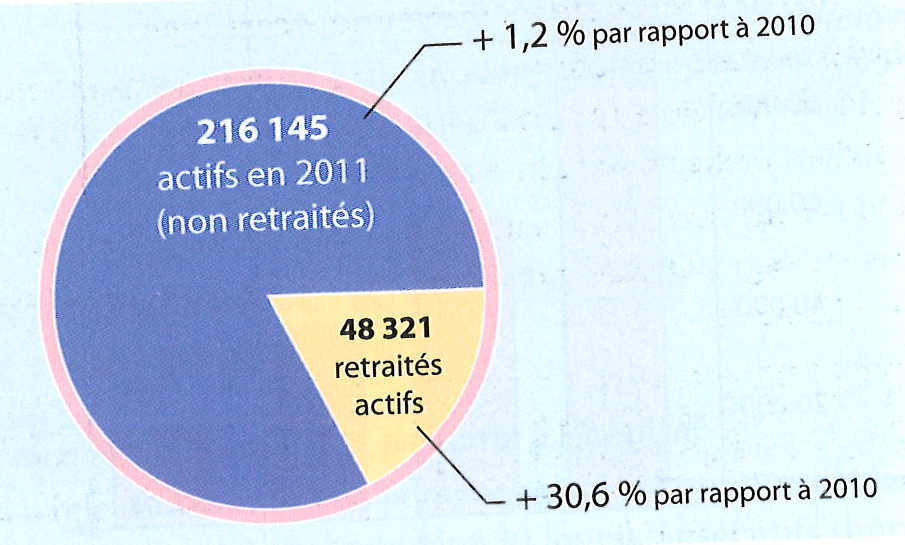
\includegraphics[scale=0.5]{repartition}
		\caption{Répartition des médecins actifs en 2011}
		\label{fig:repartition}
	\end{center}
\end{figure}


\begin{questions}
	\question Quel pourcentage de l'ensemble des médecins actifs représentent les médecins retraités en 2011 ? Arrondir à \num{0.1} \%.
	
	\question Déterminer le nombre de médecins actifs non retraités en 2010.
	
	\question Déterminer le nombre de médecins actifs retraités en 2010.
	
	\question Déterminer l'augmentation en pourcentage du nombre de médecins actifs entre 2010 et 2011. Arrondir à \num{0.1} \%.
	
\end{questions}

\subsection{Les modes d'exercice}

\begin{questions}
	
	\question Le diagramme de la figure \ref{fig:mode_exercice1} donne la répartition des modes d'exercice des médecins actifs inscrits au conseil de l'ordre en 2011. Déterminer l'effectif pour chacun des modes d'exercice.
	
	\begin{figure}{h}
		\begin{center}
			%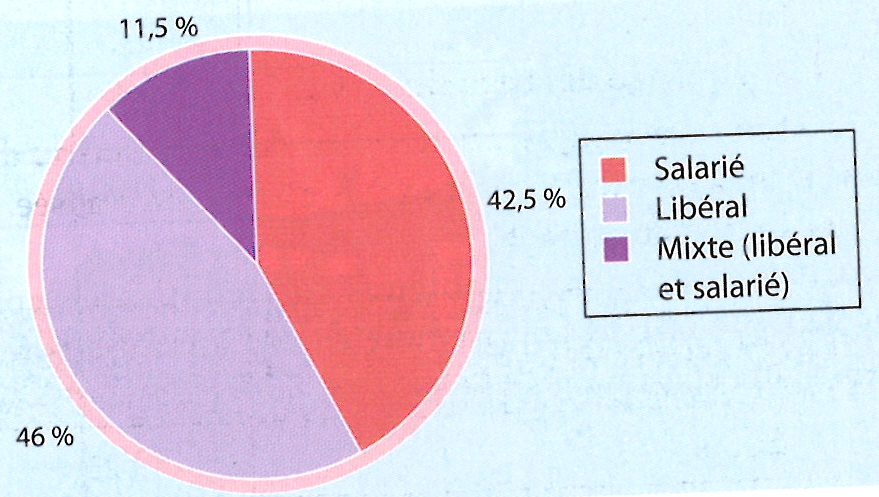
\includegraphics[scale=0.5]{mode_exercice1}
			\caption{Modes d'exercice des médecins actifs en 2011}
			\label{fig:mode_exercice1}
		\end{center}
	\end{figure}
	
	\question Le diagramme de la figure \ref{fig:mode_exercice1} donne la répartition des modes d'exercice des \num{27774} médecins de moins de 40 ans en 2011. Donner l'effectif pour chacun des modes d'exercice.
	
	\begin{figure}{h}
		\begin{center}
			%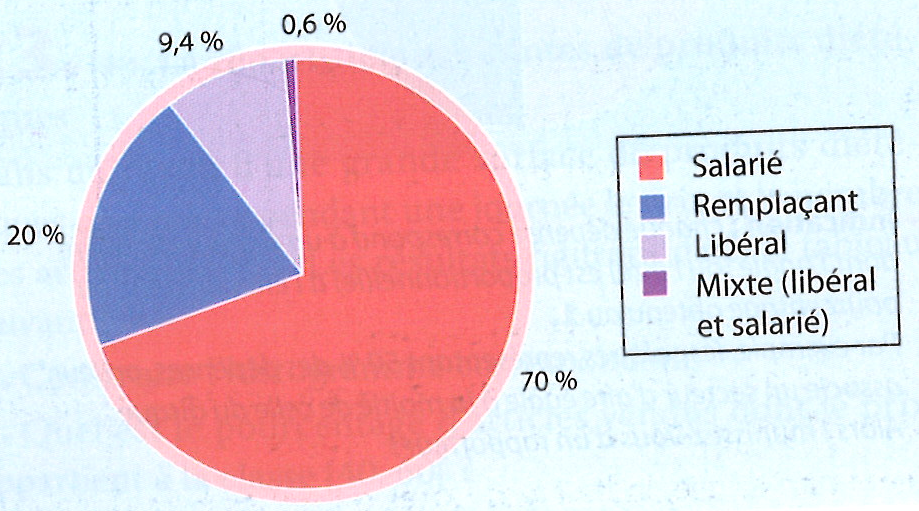
\includegraphics[scale=0.5]{mode_exercice2}
			\caption{Modes d'exercice des moins de 40 ans en 2011}
			\label{fig:mode_exercice2}
		\end{center}
	\end{figure}
	
	
	\question Quel commentaire peut-on faire sur les modes d'exercice des médecins actifs ?
\end{questions}

%\newpage

\section{Implantation d'éoliennes \textit{(12,5 points)}}

Les parties \ref{part:site_M} et \ref{part:site_F} sont indépendantes.

Après étude, les autorités d'une ile isolée ont décidé d'installer une éolienne pour répondre aux besoins énergétiques de leur communauté. L'éolienne choisie fonctionne lorsque le vent atteint au moins 8 n\oe uds et il faut l'arrêter lorsque le vent atteint ou dépasse les 48 n\oe uds. 

\subsection{\'Etude des vitesses du vent sur le site M \textit{(7 points)}}\label{part:site_M}

Les autorités décident de mesurer pendant un mois, à l'aide d'un anémomètre, la vitesse du vent sur le site M, au sommet d'une montagne. Une mesure est effectuée chaque jour.

Les résultats obtenus sont présentés dans la tableau de la figure \ref{tab:site_M} (le mois comporte 30 jours) :

\begin{figure}[h]
	\begin{center}
		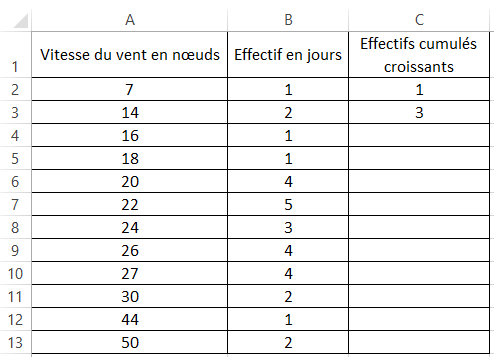
\includegraphics[scale=0.8]{eoliennes2}
	\end{center}
\caption{\'Etude de la vitesse du vent sur le site M}
\label{tab:site_M}
\end{figure}

On peut y lire que la vitesse de 22 n\oe uds a été mesurée 5 jours.

\begin{questions}
	\question[3]
		\begin{parts}
			\part[1] Compléter le tableau.
			
			\part[1] Donner une formule à placer en \textbf{\texttt{C3}} permettant, par recopie vers le bas, de calculer les effectifs cumulés croissants des jours du mois étudié.
			
			\part[1] Calculer le pourcentage des jours du mois étudié où l'éolienne ne produirait pas d'électricité. 
		\end{parts}
	
	
	\question[2] Déterminer l'étendue, la médiane, les quartiles et l'écart interquartile de cette série statistique.
	
	\question[1] On appelle premier décile (noté $D_1$) la plus petite valeur de la vitesse du vent, telle qu'au moins 10 \% des valeurs de la série sont inférieures ou égales à $D_1$. On appelle neuvième décile (noté $D_9$) la plus petite valeur, telle qu'au moins 90 \% des valeurs de la série lui sont inférieures ou égales.
	\begin{parts}
		\part[\half] Expliquer pourquoi $D_1$ = 14.
		\part[\half] Déterminer $D_9$.
	\end{parts} 
	
\end{questions}

\subsection{\'Etude des vitesses du vent sur le site F \textit{(2 points)}}\label{part:site_F}

Un emplacement sur une falaise, appelé site F, a également été retenu. Le même mois que le site M, on a mesuré les vitesses du vent sur le site F.

La série des mesures effectuée est dans le diagramme en boite de la figure \ref{fig:comparaison}. Les extrémités du diagramme correspondent aux premiers et neuvième déciles.

\begin{questions}
	
	\question[1] Lire sur le graphique les quartiles de cette nouvelle série.
	
	\question[1] Calculer l'écart interquartile.
\end{questions}

\begin{figure}[h]
	\begin{center}
		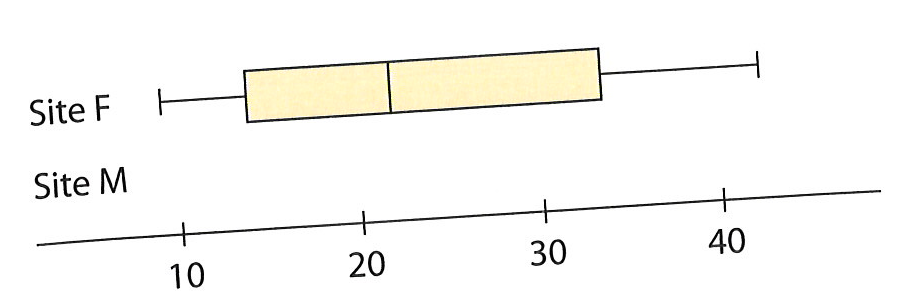
\includegraphics[scale=1.2]{moustache}
	\end{center}
	\caption{Coparaison de la vitesse du vent sur les deux sites}
	\label{fig:comparaison}
\end{figure}

\subsection{Comparaison des sites \textit{(3,5 points)}}\label{part:comp}

\begin{questions}
	\question[1\half] Représenter au-dessous du diagramme en boite fourni figure \ref{fig:comparaison}, celui de la série correspondant au site M. Prendre comme extrémités les premier et neuvième déciles.
	
	\question[2] En comparant les diagrammes, sachant qu'une éolienne a un rendement optimal aux alentours de 23 n\oe uds, quel site paraît le plsu intéressant pour l'installation de l'éolienne ? Argumenter la réponse. 
\end{questions}
	\label{LastPage}
	

\end{document}